%%%%%%%%%% Conference Latex Template for the university center of Tipaza - Algeria
%%%%%%%%%% created by F.CHABNI




\documentclass{IEEEtran}
\usepackage{graphicx}
\usepackage{amsmath}
\usepackage{cite}
\usepackage{hyperref} % add this line to your preamble
\usepackage{booktabs}
\usepackage{graphicx}
\usepackage{cite}
\usepackage{subfigure}
\markboth{Machine Learning-Powered Accident Prediction for the Automotive Insurance Industry}{Arakelyan \MakeLowercase{\textit{et al.}}: Title}



\usepackage[T1]{fontenc}
\usepackage[utf8]{inputenc}
\author{Dawid Arakelyan \\ BS in Data Science American University of Armenia Yerevan, Armenia\\ dawid\_arakelyan.\@edu.aua.am\\[1cm]{\small Advisor: Aram Butavyan\\ American University of Armenia Yerevan, Armenia}}
\title{Machine Learning-Powered Accident Prediction for the Automotive Insurance Industry}

\begin{document}
\maketitle





\tableofcontents

\ 

\begin{abstract}
Predicting car accidents is a critical issue for the insurance industry. The rise of machine learning (ML) has provided companies with new tools to analyze data and predict potential accidents more accurately. This study applies different  ML models to analyze the data from one of the Armenian insurance companies. The dataset provides car accident records and details such as car specifications. The ML algorithms used in this study include Logistic Regression, Random Forest, Xgboost, and Artificial Neural Networks (ANN). The results were evaluated using various performance metrics such as accuracy, precision, recall, and F1 score. The study showed that XGBoost and ANN outperform other models and can help to improve the accuracy of risk assessments for policy offerings.
\end{abstract}
{Key Words:}
Machine learning - XGboost -  Car accident prediction

\section{Introduction}

Car accidents are a major public safety concern worldwide, causing significant loss of life, disability, and financial struggles. According to the World Health Organization (WHO), more than 1.35 million people yearly lose their lives in road traffic accidents, with an additional 50 million suffering non-fatal injuries (WHO, 2021). In the United States alone, car accidents are the leading cause of death among people aged 1-54 (CDC, 2020). The National Safety Council (NSC) estimates that the total cost of motor vehicle deaths, injuries, and property damage in the US in 2019 was \text{\$}463.5 billion, approximately 2,5 \text{\%} of the entire US GDP (NSC, 2021). 

As a small country located in the South Caucasus region of Eurasia, with a population of around 2.9 million people, car accidents are also a significant issue for Armenia, with over 79,014 accident claims reported in 2022 alone, resulting in 3,182 human injuries (Bureau, 2022). The financial impact of car accidents in Armenia is also considerable, with the total cost of accidents in 2022 reaching approximately 15,6 billion AMD (Bureau, 2022). Having only non-life insurance in Armenia, car insurance policies can cover medical expenses, vehicle repair costs, and other accident-related expenses, reducing the financial strain on those involved. The total amount of car insurance premiums collected in 2022 was around 26,5 billion AMD. This represents a 15.6\text{\%} increase compared to the previous year (Bureau, 2022). The Armenian car insurance market is regulated by the Central Bank of Armenia and the Bureau, and it is divided into two types of insurance: compulsory and voluntary (Fitch Ratings, 2021). Compulsory car insurance is required by law and covers third-party liability, while voluntary car insurance provides additional coverage, such as comprehensive coverage, collision coverage, and theft protection (OECD, 2018). Originally  Compulsory Motor Third Party Liability Insurance (CMTPL) was introduced in 2011 as mandatory insurance for any vehicle and was controlled by the Armenian Motor Insurers Bureau. This meant that as a controlling body the Bureau was responsible for calculating the premiums Insurance companies could charge drivers for their provided service. Because of this, despite being in the market for a decade, CMTPL insurance product remains one of the least profitable for insurance companies in Armenia. Moreover, customers' dissatisfaction with this product has been consistently high as companies wanted to avoid relocating profit from other products on CMTPL while earned premiums were not enough to cover all the expenses and compensations. The loss ratio for CMTPL, which represents the paid compensation divided by the earned insurance premium, has never been stable, reaching 66\text{\%} for 2022, compared to 80\text{\%} for the same period in 2021. According to industry standards, insurance premiums should cover 75-78\text{\%} of compensation and the remaining 22-25\text{\%} for administrative expenses and income deductions.

As of April 1st, insurance companies in Armenia have been permitted to calculate premiums for insurance policies independently. This change has the potential to make the insurance market more flexible, with customized pricing for individuals, which can increase customer satisfaction. Moreover, it can foster better competition among insurance companies, leading to more innovative insurance products and services, as well as improved overall market profitability. Therefore, this new development could be a turning point for the Armenian insurance market, providing an opportunity for growth and improvement in the coming years. Based on this all companies can create their own pricing models based on their predictions and business calculations. Here comes the help of Machine learning models that can facilitate in this by predicting the likelihood of an accident occurring and identifying the factors that are most strongly associated with accidents. By analyzing car accident data and identifying trends and patterns, we can gain insights that can change the way of defining prices for contracts. One area where machine learning has been applied is in predicting car accidents and insurance claims. The focus of this capstone project will be to develop a machine-learning model to predict the likelihood of car accidents in Armenia based on various factors, such as vehicle details, driver history, personal characteristics, and more. The model will be trained on a dataset of car accidents in Armenia from the past several years, and we will use various machine-learning algorithms to identify the most accurate model.




\section{Literature Review}
There have been several studies examining the performance of different machine learning models in predicting car accidents and insurance claims. In the study "A Comprehensive Study of Car Accident Prediction Models Using Machine Learning Techniques'' by M. A. Al-Quraishi and S. S. Al-Rawashdeh, numerous machine learning algorithms were evaluated and compared for their performance in predicting car accidents. It considered a dataset from the Arizona Department of Transportation containing information on car accidents between 2016 and 2017. The performance comparison of various machine learning algorithms, including logistic regression, decision tree, random forest, and support vector machine showed that random forest and decision tree algorithms outperformed the other models with an accuracy of 89.8\text{\%} and 87.6\text{\%}, respectively. The study also concluded that weather conditions and traffic volume were the most significant factors in predicting car accidents. In a study by Smith et al. (2000), several machine learning models were tested to assess whether policyholders submit a claim or not. The tested models included decision trees and neural networks. The study found that the neural network model performed better than the decision tree model. Similarly, Weerasinghe and Wijegunasekara (2016) compared decision trees, artificial neural network, and regression models and  as a result indicating that the artificial neural network model was the best predictor of claim severity. In a recent study by Pesantez-Narvaez et al. (2019), two competing methods, XGBoost and logistic regression, were used to predict the frequency of motor insurance claims. The study indicated that the XGBoost model was slightly better than logistic regression. Another paper, "Comparative Study of Machine Learning Models for Prediction of Car Accidents" by S. Sharma, R. K. Yadav, and M. Singh, evaluated and compared the performance of four machine learning algorithms: Logistic Regression, Decision Tree, Random Forest, and Gradient Boosting Machine. The authors found that GBM performed the best, with an accuracy of 93.7\text{\%}, followed by RF, with an accuracy of 92.2\text{\%}. DT and LR showed lower accuracy levels of 86.7\text{\%} and 80.\text{\%} respectively.  Analysis of several related works showed that various weather-related variables can be effective in predicting car accidents accurately. For instance, a study by Lee et al. (2017) used data on weather conditions particularly temperature, visibility, wind speed, and precipitation to develop a predictive model. The study found that low visibility, high precipitation, and low temperature were all significant predictors of accidents. In another study, Chen et al. (2017) utilized traffic volume, speed, and road geometry data and showed that high traffic volume and speed significantly affect the likelihood of accidents additionally being a considerable  predictor. Driver age is generally considered to be at higher risk of accidents due to their lack of experience and more impulsive behavior. As Prato Prato et al. (2016) showed, drivers aged 18-24 were more likely to be involved in car accidents than older drivers. Moreover, male drivers in this age group were at even higher risk. The location where a driver resides can also affect their likelihood of being involved in an accident (Jovanis et al. (2015). Besides these metrics, the driver's type of car can also impact the potentiality of accidents; specifically SUVs and minivans were less likely to be involved in accidents and had better driving techniques (Quddus et al.,2015) . These are just a few examples of the features that have been used in prediction of car accidents using machine learning. Different studies may use different variables and approaches based on their specific research question. However, these key features are widely recognized as essential factors that can significantly impact the possibility of accidents. In terms of car insurance prediction, these features can be used to assess the risk of insuring a driver and determine the appropriate premiums.
Feature engineering involves selecting the relevant features from the available data, transforming them into a suitable format, and combining to create new features that can improve the model's performance. A study published in the Journal of Safety Research by Liu et al. (2019)  collected driving behavior data from 1,000 drivers in China and used it to create features such as average speed, acceleration frequency, and brake frequency. This data then was combined t with accident reports to develop a machine learning model that could predict the risk of accidents based on driving behavior. The results showed that the model had an accuracy of 82.3\text{\%}, demonstrating the effectiveness of combining car usage and accident data for accident prediction. 

Data cleaning involves identifying and correcting errors and inconsistencies in the data, which can significantly affect the performance. The study by El-Basyouny et al. (2020) collected accident data from the city of Toronto and used different cleaning methods among which  Z-score and Tukey's method, to remove outliers from the data. They then trained machine learning models on the cleaned data and compared their performance to models trained on uncleaned data. The results showed an improved accuracy of 6\text{\%} in machine learning models when removing outliers .

\section{Background }

To be able to predict car accidents based on drivers' behavior, it is crucial to have an understanding of several topics like insurance claims forecasting, data cleaning and organization, feature engineering, machine learning, and classification. Starting with analyzing the data from insurance claims and contracts, it's important to clearly understand what kind of data might be helpful to be used during the later processing. With a vast amount of data available to determine the likelihood of claims occurrence, it is necessary to utilize big data models. A reliable and effective approach using machine learning models will be used to assess the potential risk that a driver poses to an insurance provider and the probability of them filing a claim in the upcoming year. Such model must be capable of analyzing and interpreting extensive databases comprising thousands of consumer details provided by Sil Insurance. Using the given opportunity, data taken from one of the main insurance companies, personalized insurance quotes are based on a driver's ability, and they believe that employing effective techniques can yield more accurate predictions of claims occurrence. For this purpose, two different datasets were taken where; one contains details about a driver, his car, and contract, and the other contains data regarding car accidents. Together, more than 500.000 rows of information were collected, representing several years.

\

\subsection{Machine learning and Accident prediction}


Predicting car accidents is a complex task that requires the use of various metrics as target variables. A plethora of machine learning algorithms can be applied to achieve the goal of predicting the likelihood of accidents, including linear models, decision trees, clustering, or classification models (Nguyen et al. 2017). However, the most appropriate model for the task should be chosen based on the specific characteristics of the dataset.

The predictive problem can be described by a vector of predictor variables $x = \{x_1, \ldots, x_p\}$ and an output or target variable $y$. The input variables are represented by a group of quantitative and qualitative features of the automobile and the policyholder, and the result is the actual accident claim prediction. Given a group of $M$ instances $\{(y_i, x_i); i = 1, \ldots, M\}$ of known $(y, x)$ values, the purpose is to use the given data to obtain an estimate of the function that maps the input. In this case, the target variable was transformed into a binary one, with the value 0 representing no accident and the value 1 representing an accident occurrence.
\begin{center}
    $Y = \{0,1\}$ 0\
\end{center}

\begin{center}
    $Pr(Y = 0|X = x_i)$\hspace{1 cm} $Pr(Y = 1|X = x_i)$ \\
\end{center}



$X$ is a collection of instances $x_i$ that represents all of the known information of the $i$-th policyholder.

Therefore, the problem can be identified as a binary classification, where the aim is to predict the probability of claim occurrence (Kotsiantis et al. 2006). Moreover, the use of feature engineering techniques can enhance the accuracy of the classification model. In their study, Nguyen et al. applied feature engineering techniques to improve the performance of the classification model in predicting car accidents. The study showed that feature engineering techniques, such as feature scaling and feature selection, can increase the accuracy of the model by reducing the number of irrelevant features and scaling the features to the same range.

\

\subsection{Logistic regression}

Logistic regression is a statistical method for analyzing a dataset in which there are one or more independent variables determining an outcome. It is commonly used in binary classification problems where the outcome variable is binary (e.g., yes or no, 0 or 1). The goal of logistic regression is to find the best fitting model to describe the relationship between the independent and dependent variables. This model uses a logistic function to model the probability of the outcome variable. The logistic function is an S-shaped curve that transforms any real-valued input to a value between 0 and 1, representing the probability of the outcome variable being in one of the two classes. The function is defined as:

\begin{equation}
P=\frac{e^{a+b X}}{1+e^{a+b X}}
\end{equation}

One limitation of logistic regression is that it assumes a linear relationship between the independent variables and the logit of the outcome variable. Non-linear relationships may require more complex models to accurately predict the probability of the outcome variable.


\\
\
\subsection{Decision trees}

Decision trees are a type of supervised machine learning algorithm that can be used for classification and regression tasks. They are constructed by recursively partitioning the input space into smaller regions, where each partition corresponds to a node in the tree. 

\

\begin{figure}[h]
\centering
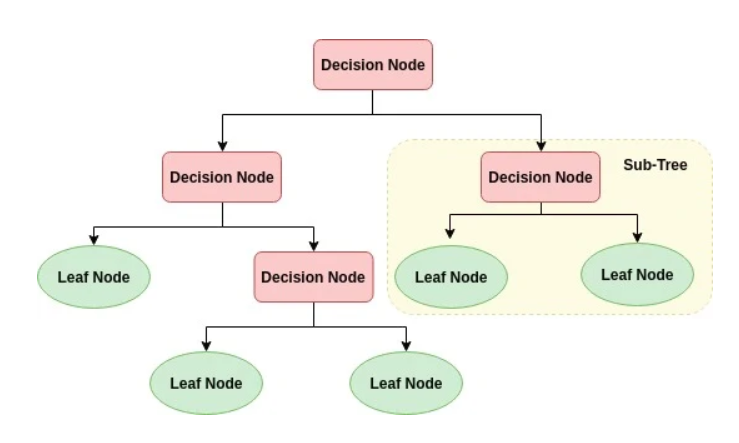
\includegraphics[width=0.5\textwidth]{df.png}
\caption{\label{fig:dt}Decision Tree workflow.}
\end{figure}

\
The goal of this partitioning process is to minimize the impurity of the target variable within each region so that the resulting tree can accurately predict the target variable for new data points (Quinlan, 1986). One of the advantages of decision trees is their interpretability, as the resulting tree structure can be easily visualized and understood by humans (Murthy, 1998). They are also relatively fast to train and can handle both numerical and categorical data (Kotsiantis et al., 2007). However, decision trees can suffer from overfitting, which can be mitigated by pruning techniques or by using ensemble methods such as random forests (Breiman, 2001). Overall, decision trees are a versatile and widely-used machine learning technique with applications in fields such as finance, healthcare, and environmental science (Boriah et al., 2012; Alemzadeh et al., 2016).

\subsection{Random Forest}

The Random Forest algorithm is based on the concept of decision trees, where a tree-like model is constructed to make predictions by recursively splitting the data based on certain criteria. In the Random Forest algorithm, multiple decision trees are created using different subsets of the data and different sets of features. This process is known as bagging or bootstrap aggregating. The algorithm then combines the predictions of the individual trees to make the final prediction. One of the main advantages of Random Forest is its ability to handle a large number of features and still avoid overfitting (Breiman, 2001). The algorithm also has high accuracy and is relatively fast to train. The Random Forest algorithm has been used in various studies for car accident prediction and has shown promising results(Wu et al., 2017). For instance, in a study by Abbas et al. (2019), the Random Forest algorithm was used to predict car accidents based on driver characteristics, and as a result, it outperformed other machine learning algorithms such as SVM and KNN. In another study by Wu et al. (2017), the Random forest was compared to other machine learning models for the same task, and again the results showed that it outperformed other models in terms of accuracy and F1 score.

\subsection{XGBoost}

XGBoost is a popular machine-learning algorithm that has gained a lot of attention in recent years due to its high accuracy and efficiency. It is a gradient-boosting framework that can be used for both classification and regression tasks. The XGBoost algorithm was first introduced in 2014 by Tianqi Chen and Carlos Guestrin in the paper "XGBoost: A Scalable Tree Boosting System" (Chen and Guestrin, 2016).
XGBoost works by iteratively adding decision trees to an ensemble, with each tree attempting to correct the errors made by the previous tree. During each iteration, the algorithm calculates the gradients and Hessians of the loss function with respect to the predicted values and then fits a tree to the negative gradient. The trees are added sequentially until the specified number of trees or a stopping criterion is reached. One of the main advantages of XGBoost is its ability to handle missing data, as well as its regularized learning approach, which helps to prevent overfitting. Additionally, XGBoost has a number of tuning parameters that can be adjusted to optimize its performance for specific datasets. In terms of performance, XGBoost has been shown to outperform many other popular machine learning algorithms on a variety of datasets, including the Kaggle data science competition platform (Chen and Guestrin, 2016). It is often considered one of the most preferred algorithms for many data science and machine learning projects due to its high accuracy, speed, and ease of use.

\

\begin{figure}[h]
\centering
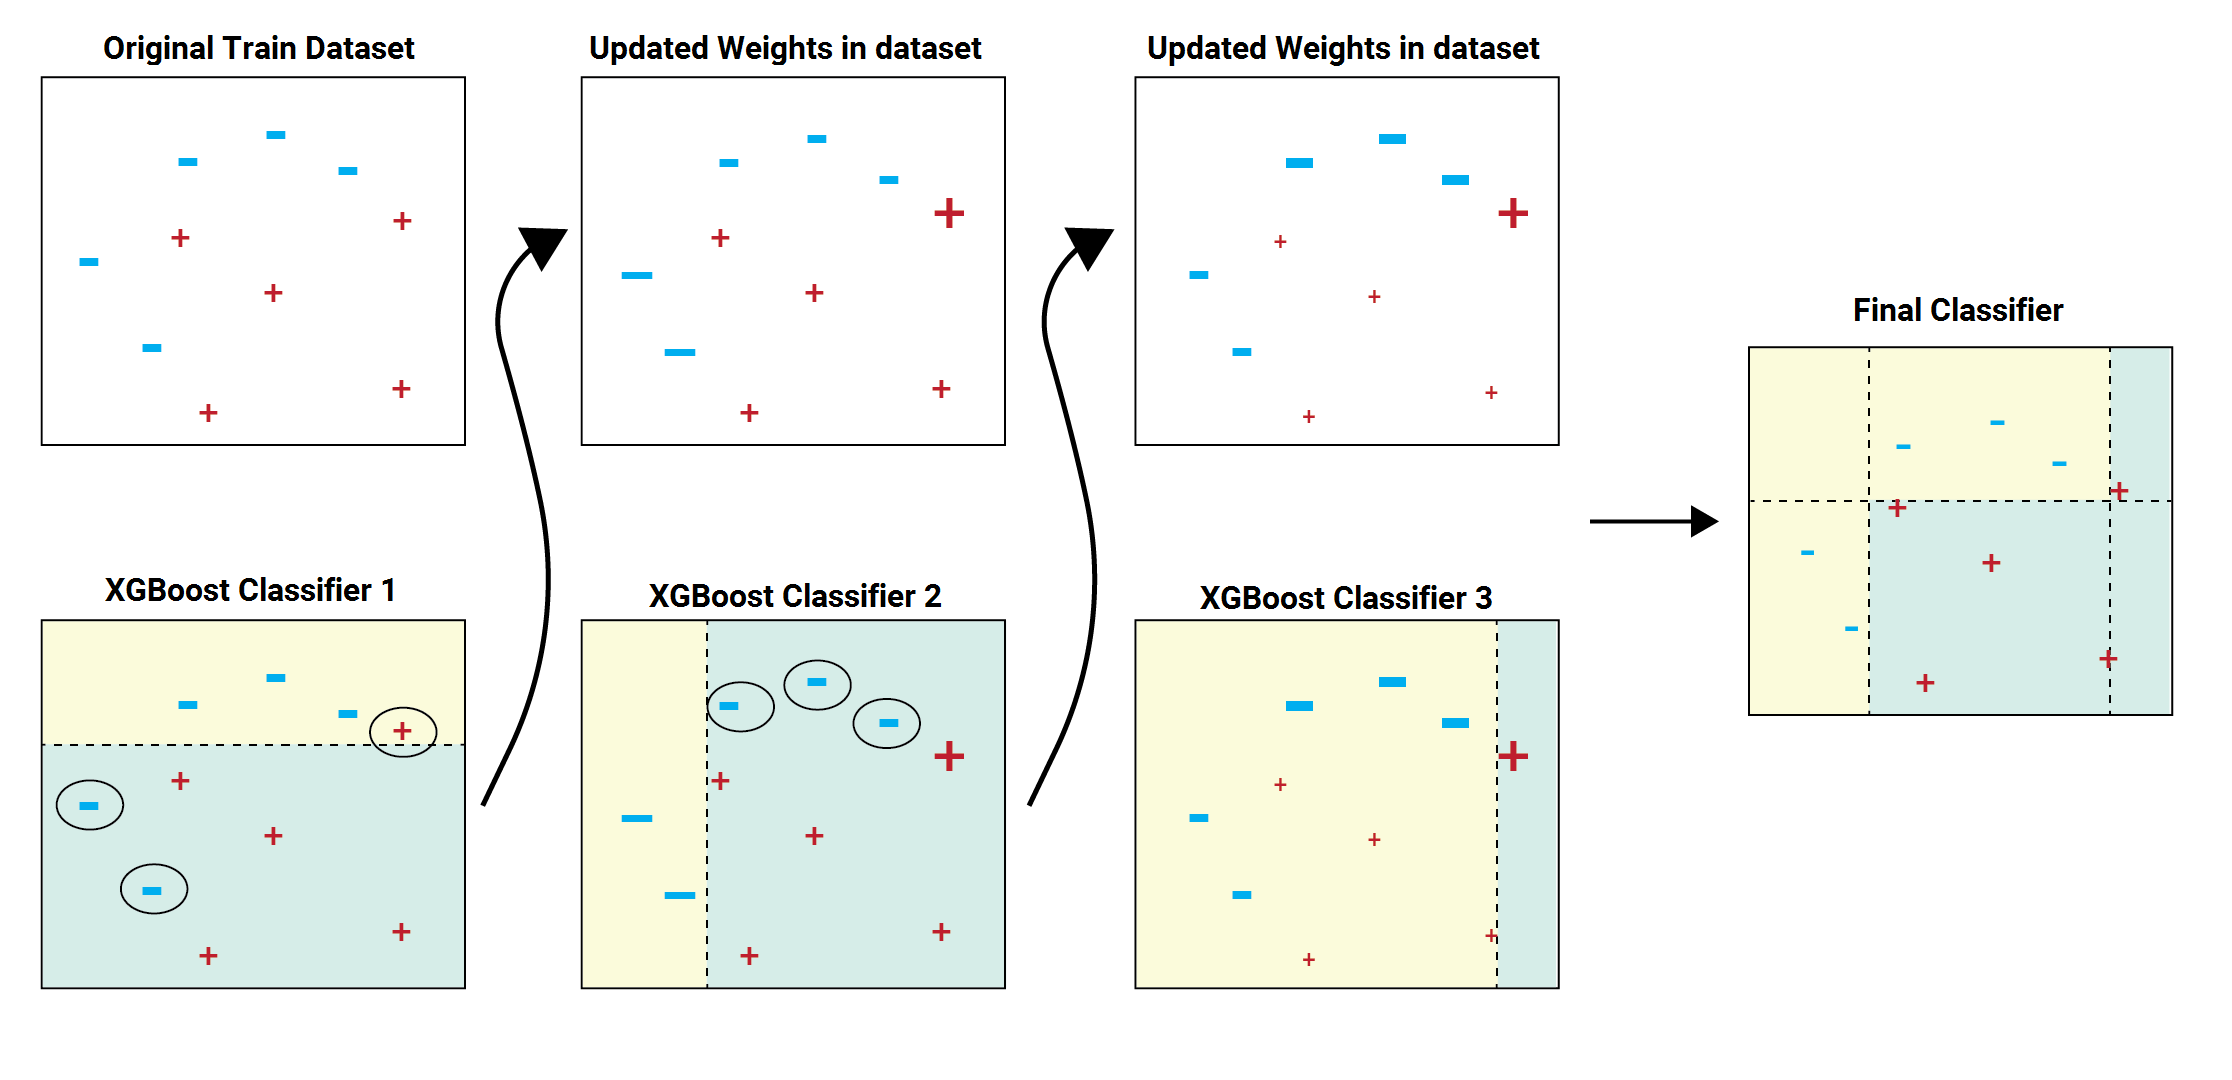
\includegraphics[width=0.35\textwidth]{XG-Boost-FINAL-01.png}
\caption{\label{fig:xgb}XGBoost workflow.}
\end{figure}


\subsection{Artificial neural networks}

Artificial neural networks (ANNs) are a machine learning algorithm inspired by the structure and function of the human brain. ANNs consist of multiple layers of interconnected nodes (neurons) that perform complex mathematical operations on input data to generate an output. ANNs are capable of learning complex patterns and relationships in data and are commonly used in various fields, including image and speech recognition, natural language processing, and predictive modeling. ANNs can model non-linear relationships between inputs and outputs. This makes them particularly useful in situations where the relationship between variables is not easily modeled using linear regression or other traditional statistical methods. ANNs are also robust to noise and can handle missing data, making them a suitable choice for many real-world applications.


\begin{figure}[h]
\centering
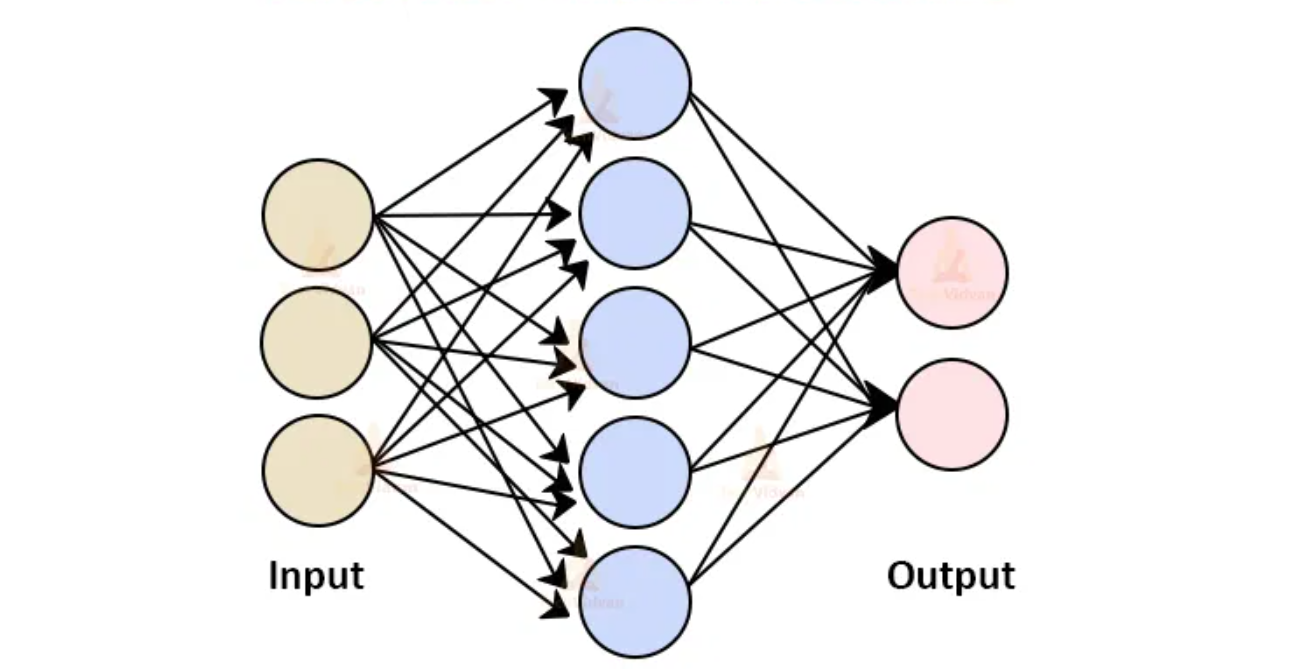
\includegraphics[width=0.2\textwidth]{ann.png}
\caption{\label{fig:ann}ANN workflow.}
\end{figure}


\section{Dataset}

In this study, I have worked with two datasets obtained from the SIL Insurance database. The first dataset contains information about approximately 550,000 general contracts, while the second dataset contains information about approximately 32,000 accidents. Both datasets contain real data from actual customers and accidents, making them highly relevant and informative for analysis. These datasets offer a wealth of information about customer behavior, contracting processes, and accident occurrences. By analyzing these datasets, I aim to attain valuable insights into the company's operations and customers, additionally develop targeted interventions to make an accurate prediction. Some initial data preparation was performed using Excel. This included tasks such as separating months by horoscope signs, deleting wrong columns, etc. These steps helped to ensure that the data was ready for analysis in pandas and reduced the amount of cleaning required within the Python environment.

\subsection{Contract Data}

The first dataset originally contained 28 columns, with about half of them being irrelevant to the analysis. The most important columns in the dataset include information about the drivers, such as their age, horoscope, and gender, as well as information about the cars, such as the make, model, age, and other contract-related details including start and end dates.

Unprocessed Columns
\begin{itemize}
\item Id: An identification number for each contract in the dataset (number)
\item Car: The brand of the car for the given contract (BMW, Opel,etc.)
\item Hp: The horsepower of the car (number)
\item User id: A unique identification number for each customer (number)
\item texttt{Cont\_Start}: The start date of the insurance policy (datetime)
\item texttt{Cont\_End}: The end date of the insurance policy (datetime)
\item texttt{Cont\_Days}: The number of days the insurance policy was active (number)
\item Year: The year policyholder was born (12 astrological ages)
\item Month: The month policyholder was born (12 zodiacal signs)
\item Region: The region where the customer resides (11 provinces of Armenia)
\item Root: The way the contract was signed (online, offline, agent)
\item Gender: The customer's gender (male, female)
\item Type: The type of insurance policy for the car (Car, Truck, Moto)
\end{itemize}

\
Processed Columns
\begin{itemize}
\item Model: The model of the car (processed into texttt{Car\_class} column)
\item texttt{Car\_class}: The car categorization based on the class (A, B, C, SUV, etc.)
\item Plate: The license plate number of the car (processed into Group column)
\item Group: The price group representing each license plate (1-12)
\item texttt{Car\_year}: Age of the car when the contract started (number)
\item texttt{D\_age}: The age of the customer in years (18-200)
\item Target: Whether or not the insurance policy resulted in a claim (0 or 1)
\end{itemize}

\begin{figure}[h]
\centering
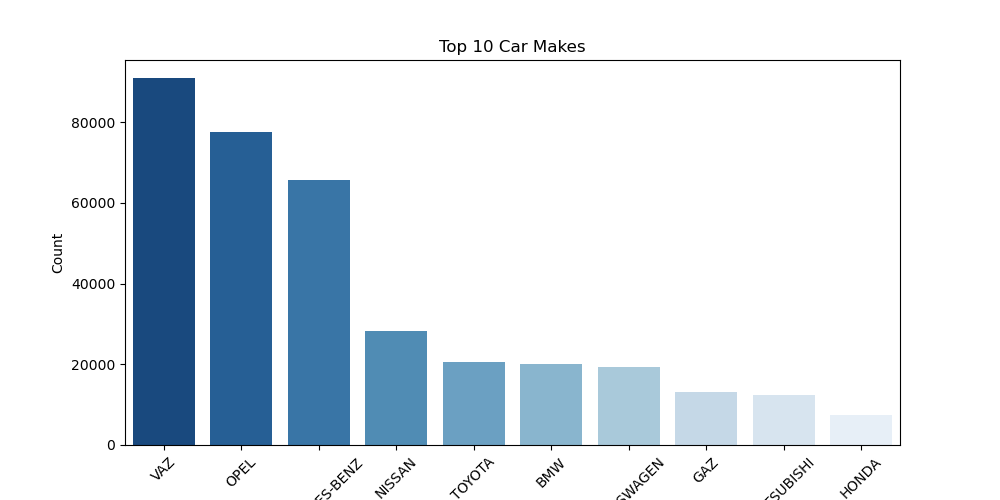
\includegraphics[width=0.5\textwidth]{top_car_makes.png}
\caption{\label{fig:top}Top 10 car makes }
\end{figure}

\begin{figure}[h]
\centering
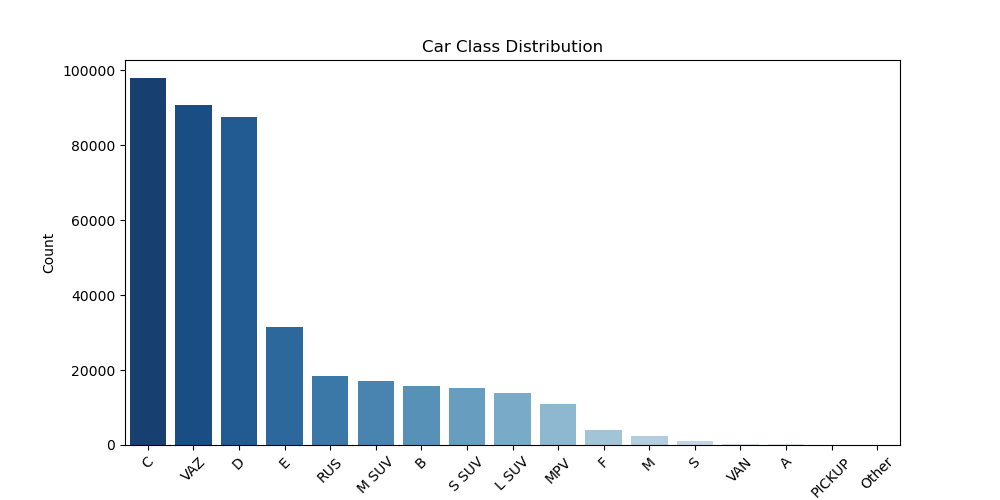
\includegraphics[width=0.5\textwidth]{car_class_distribution.png}
\caption{\label{fig:ccd}Car Class Distribution  }
\end{figure}


Contracts with a driver's age lower than 18 or higher than 200 were dropped, and the rows with empty values were in the "Car" column. Later, Car brands that appeared less than 84 times in the entire dataset were removed to avoid adding too many categorical variables to the dataframe.  Around 7500 missing values in the "model" column were imputed by matching the car's brand and horsepower with those of other cars in the dataset, and then assigning the missing model the same value as the matched cars. Data processing involves transforming the "model" column in the dataset into a categorical variable that can be used for modeling. This was done by creating a new column called "Car-class" based on the car's brand and model. The car models were grouped into representative car classification groups based on certain criteria, such as the car's size, features, and performance. This process makes it easier to analyze and model the data, as the car models are now represented by a categorical variable that can be used as an algorithm input feature. The plate numbers were grouped by prices, with information about the groups being scraped from 
\href{https://roadpolice.am}{Road Police}, to ensure no groups were missed.  Ultimately, the plate numbers were categorized into 12 groups, with the first group representing the free plate numbers and the most expensive group being labeled as group 12. All the plates not having the standard form were dropped. The driver's bd column has been transformed into age based on the contract dates and similarly transformed, the car age column. Additionally, the column representing driver payoffs during the contract was converted into a binary column, with 1 indicating at least one payoff and 0 indicating no payoffs. This column is going to be used later as a target column. These normalization steps ensured the data was standardized and could be effectively analyzed in the capstone project. These data cleaning and prepossessing steps have helped to ensure that the relevant data is standardized and ready for analysis in the project. 

\subsection{Accident data}

The second data frame used in the analysis was well-organized and clean, containing only the relevant columns. Specifically, it contained information related to car accidents, such as the driver's ID, contract ID, the type of damaged object involved in the accident, the date of the accident, and the amount of the resulting payout. These columns were crucial for understanding the frequency and severity of accidents, as well as the associated costs.In order to avoid duplication of data and ensure the correct merging of accidents to their respective contracts, relevant columns from the given data frame were utilized to create contract accident metrics.


\begin{itemize}
\item Id: An identification number for each contract in the dataset
\item Total-acc: Total number of accidents associated with each contract.
\item Total-dam-items: Total number of damaged items associated with each contract.
\item Payoff-amount-car: Total amount of payments made for car damage associated with each contract.
\item Payoff-amount-human: Total amount of payments made for human damage associated with each contract.
\item Payoff-amount-object: Total amount of payments made for object damage associated with each contract.
\item Dam-id-car: Total number of car damage items associated with each contract.
\item Dam-id-human: Total number of human damage items associated with each contract.
\item Dam-id-object: Total number of object damage items associated with each contract.
\item Total-payoff: Total amount of payments made for all types of damage associated with each contract.
\item Min-payoff: The minimum amount of payment made for any damage associated with each contract.
\item Avg-payoff: The average amount of payment made for any damage associated with each contract.
\item Max-payoff: The maximum amount of payment made for any damage associated with each contract.
\item Min: The date of the first accident associated with each contract.
\item Max: The date of the last accident associated with each contract.
\item First-accident-days: The number of days between the first accident associated with each contract and the current date.
\item Last-accident-days: The number of days between the last accident associated with each contract and the current date.
\end{itemize}

\begin{figure}[h]
\centering
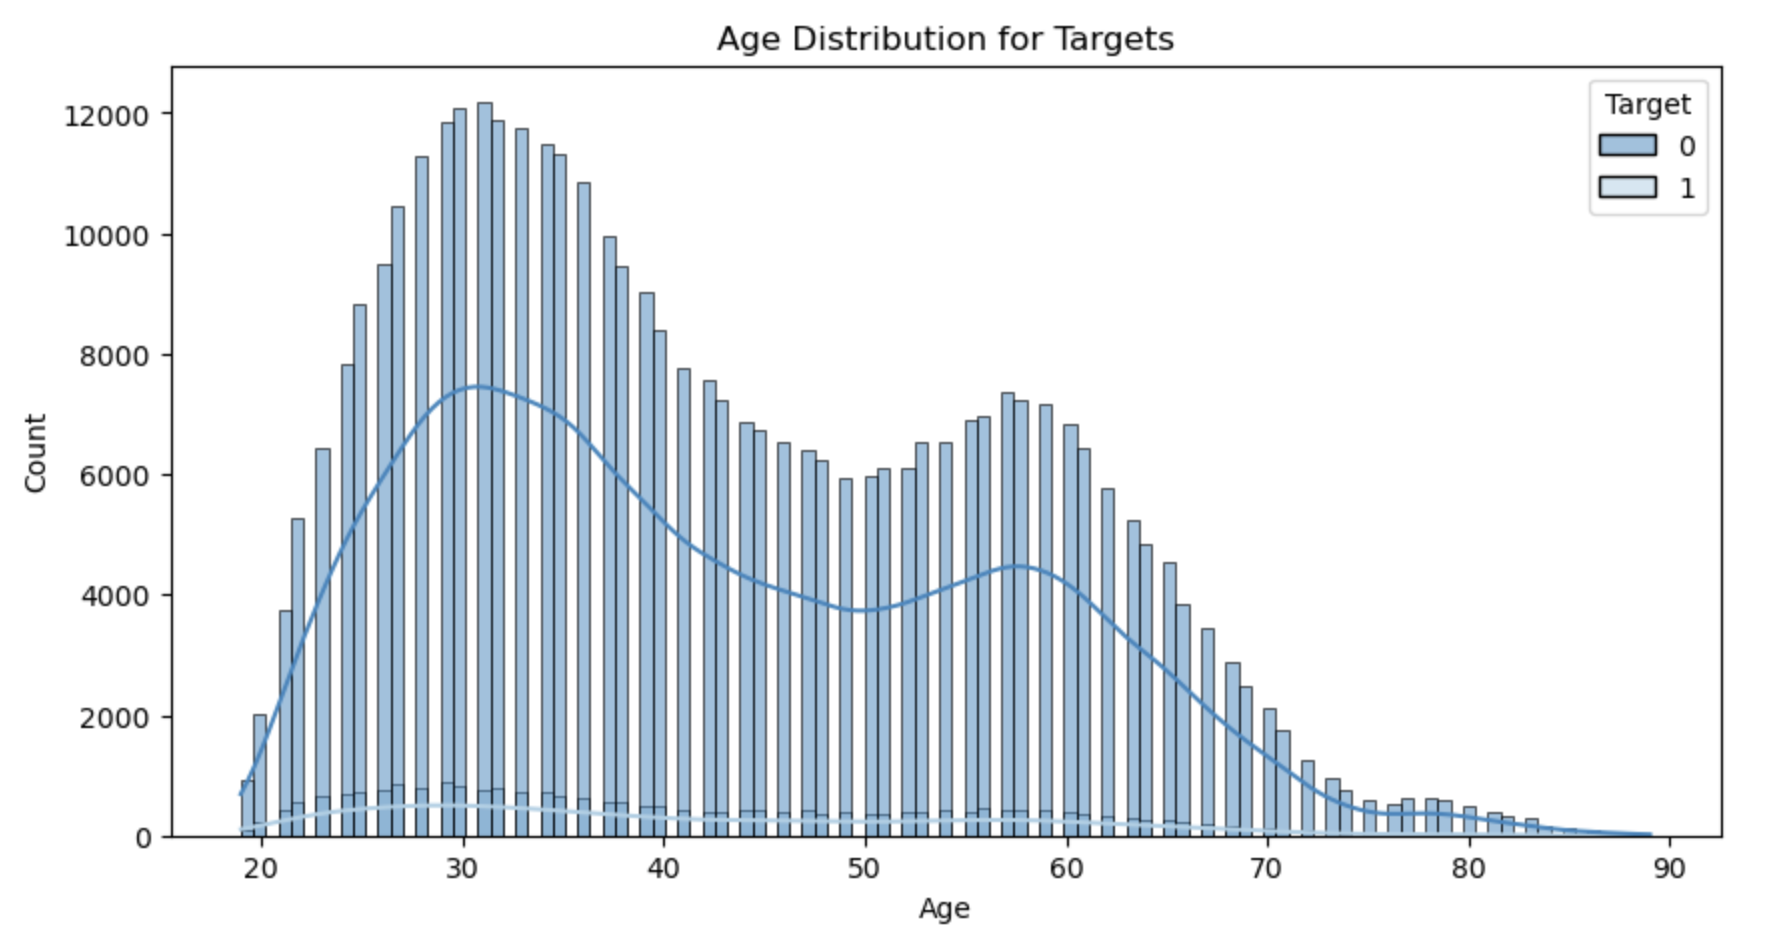
\includegraphics[width=0.45\textwidth]{age_and_target_distribution.png}
\caption{\label{fig:at}Age and Target distribution  }
\end{figure}


\subsection{Data merging}

To create a comprehensive dataset, both data frames were joined based on their shared contract IDs, resulting in a single, unified dataframe. This combined data frame included all relevant information regarding the contract, driver and their car, as well as any accidents that occurred during the contract period. Feature engineering techniques were then applied to the dataset, adding new features such as the sum of contracts taken out by a driver prior to the given contract, or the average payout per contract. 




\section{Model Evaluation  }

To assess the performance of prediction models, several evaluation metrics can be used. The most common evaluation method of the model is the accuracy score. However, for big datasets, it may not accurately represent how good the model is (biased accuracy), which means it is not reliable. The problem comes from the imbalanced data. While the accuracy score represents the total view of a model, by calculating the ratio of the outputs, minor classes might be lost in the big data sets, meanwhile being the main needed output. While looking at the dataset used for this paper, one can notice that the percentage of the two groups of the target variable are 6\text{\%} & 94\text{\%}, where 6\text{\%} represents the cases with car accidents, and the rest denotes the policies without accidents. Car insurance data is extremely imbalanced, so the usual accuracy scores are useless. Other metrics like confusion matrix, F-score, recall and precision, the area under curve (AUC), and kappa are used to overcome this issue.


\subsection{Confusion matrix}

The first tool to understand how well the binary classification of the model works is the confusion matrix. It represents how the model predicted both different classes. There are four parameters that the matrix shows. True positive (TP), True negative (TN), False positive (FP), and False negative (FN). TP and TN illustrate the amount of correctly classified positive and negative cases, while  FP and FN display incorrectly classified positive and negative instances. Within this paper, true positive value will represent no accident, and true negative will represent a car accident.



\begin{figure}[h]
\centering
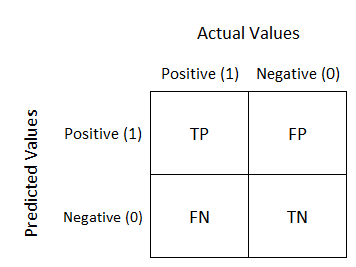
\includegraphics[width=0.5\textwidth]{tp.png}
\caption{\label{fig:tp}Confusion Matrix.}
\end{figure}

After calculating the values of the coefficient matrix, accuracy can be found. The Accuracy score is defined as a ratio of the positive values over the sum of all four elements.

\begin{center}
    $Accuracy = \frac{TP + TN}{TP + TN + FP + FN}$
\end{center}


\subsection{Precision & Recall}

The precision measures how trustworthy the type is classified, and whether it belongs to the correct class. On the other hand, the recall calculates how well the fraction of a positive class becomes correctly classified; this essentially shows how well the model can detect the class type (Hossin and Sulaiman 2015).

\subsection{F-score}

F-score, also known as F1-score or F-measure, combines both precision and recall into a single measurement. It's a ratio of precision times recall over the sum of precision and recall times 2.

\subsection{AUC - ROC}

AUC (Area Under The Curve) and ROC (Receiver Operating Characteristics) curve is an essential measurement for classification problems. It is also called AUROC (Area Under the Receiver Operating Characteristics). ROC represents a probability curve, and AUC displays the degree or measure of separability. The curve shows how well the model can differentiate classes. The higher the AUC, the better the model predicts 0 as 0 and 1 class as 1. 

\begin{figure}[h]
\centering
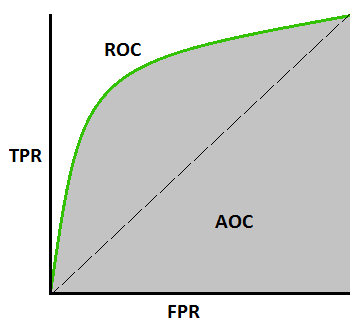
\includegraphics[width=0.3\textwidth]{auc.png}
\caption{\label{fig:auc}AUC-ROC}
\end{figure}




\section{Model }

This study aimed to develop a predictive model that can accurately predict the likelihood of car insurance claims by utilizing various machine learning approaches. The entire process involved several stages, carefully designed to ensure the accuracy and robustness of the final model. These stages included data gathering and preprocessing, feature engineering, model selection, training, and evaluation. The figure below provides a visual representation of the different steps involved in the study. 


\begin{figure}[h]
\centering
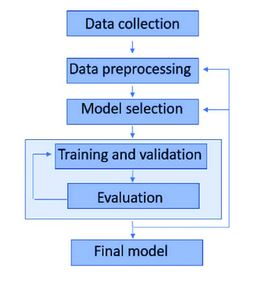
\includegraphics[width=0.3\textwidth]{mod.JPG}
\caption{\label{fig:mod}ML model workflow}
\end{figure}

\subsection{Final Data processing }

New columns were created  based on previously calculated metrics, which represent the historical performance of each driver for their contracts in the dataset. These columns provide information on the past state of various metrics for each contract associated with each user.

\begin{itemize}
\item prev-contracts: the number of contracts the user has completed before the current one
\item prev-damaged-cars: the total number of cars damaged by the user in all previous contracts
\item prev-damaged-human: the total number of humans damaged by the user in all previous contracts
\item prev-damaged-object: the total number of objects damaged by the user in all previous contracts
\item prev-payoff: the total payoff the user received in all previous contracts
\item prev-Avg-payoff: the average payoff the user received in all previous contracts
\item prev-Min-payoff: the minimum payoff the user received in all previous contracts
\item prev-Max-payoff: the maximum payoff the user received in all previous contracts
\item prev-tot-dam-items: the total number of items (cars, humans, and objects) damaged by the user in all previous contracts
\item prev-tot-acc: the total number of accidents (collisions with cars and objects) the user was involved in, in all previous contracts
\item prev-pay-cars: the total payoff the user received for damaging cars in all previous contracts
\item prev-pay-human: the total payoff the user received for damaging humans in all previous contracts
\item prev-pay-object: the total payoff the user received for damaging objects in all previous contracts
\item prev-Latest-acc: the number of days since the user's last accident as of the start of their current contract
\item prev-First-acc: the number of days since the user's first accident as of the start of their current contract
\item Previous Contracts: The number of previous contracts of a user
\item Contracts Age Factor: The age of the user's contracts.
\item Damage Frequency: The ratio of total damaged items to total accidents in previous contracts for each user.
\item Accident Severity: The severity of accidents in previous contracts for each user
\item Payoff Frequency: The ratio of total payoffs to total accidents in previous contracts for each user.
\item Average Contract Days: The average number of days of contracts for each user.
\item Score based on Accidents and Payoff: A score that takes into account the user's history of accidents and payoffs,
\item Score based on Accidents, Payoff, and Damaged Cars: A score that takes into account the user's history of accidents, payoffs, and damaged cars
\item Score based on Accidents, Payoff, and Contract Length: A score that takes into account the user's history of accidents, payoffs, and contract length
\item Driver Tenure: The length of time in years that the user has been a driver with the company
\item Overall Driver Score: A score that takes into account the user's driver tenure, history of accidents, payoffs, contract length, and damage frequency
\item Driver Score1: A score that takes into account the user's history of accidents, payoffs, contract length, and damaged cars,
\item Decay Factor1: A factor that decreases with time since the end of the current contract
\item Driver Score: A score that takes into account the user's history of accidents, payoffs, contract length, and the time since the end of the current contract
\end{itemize}


In the final dataset, we had a total of 43 columns generated by processing various metrics for each user's contract history. Out of these, 7 columns were categorical and were converted into dummy variables to be used in the model. As a result, the final dataset consisted of 148 columns and 407.278 rows. Notably, the final dataset had no empty or null values.


\subsection{Target Variable  }

The target variable in our dataset is a binary column with two classes - 1 and 0, where 1 indicates the occurrence of a claim, and 0 indicates the absence of a claim. However, the dataset suffers from severe class imbalance, with class 0 having 93.9\text{\%} observations and class 1 having only 6.03\text{\%} observations. This can affect the performance of ml algorithms, as they tend to be biased towards the majority class. To solve this problem, the technique of oversampling using the RandomOverSampler was employed. Oversampling involves generating more instances of the minority class to balance the dataset and increase the probability of the minority class. This function randomly replicates the existing instances of the minority class until it matches the number of instances in the majority class. The RandomOverSampler function in Python is a simple and effective way to address the class imbalance. 

\begin{figure}[h]
\centering
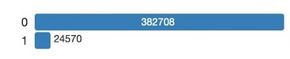
\includegraphics[width=0.3\textwidth]{bef.JPG}
\caption{\label{fig:bef}Before oversampling   }
\end{figure}

\begin{figure}[h]
\centering
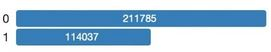
\includegraphics[width=0.3\textwidth]{af.JPG}
\caption{\label{fig:af}After oversampling   }
\end{figure}

\subsection{Correlation }

 In the correlation matrix, the heatmap shows the correlation between all pairs of features in the dataset. However, to better understand which features are most strongly correlated with the target variable, we can focus on the top 30 features with the highest correlation coefficients. This can help identify which features may be the most important predictors for the target variable. The correlation matrix shows that specific columns, such as Prevous-first-acciden, prevouse-tot-contact, Previous-payoff, and other columns related to the driver's previous experience, have a high correlation with the target variable. This suggests that feature engineering techniques effectively identified relevant predictors of the target variable. The high correlation values also indicate that these features may be strong predictors of the target variable and should be further investigated in modeling and analysis.


 

\begin{figure}[h]
\centering
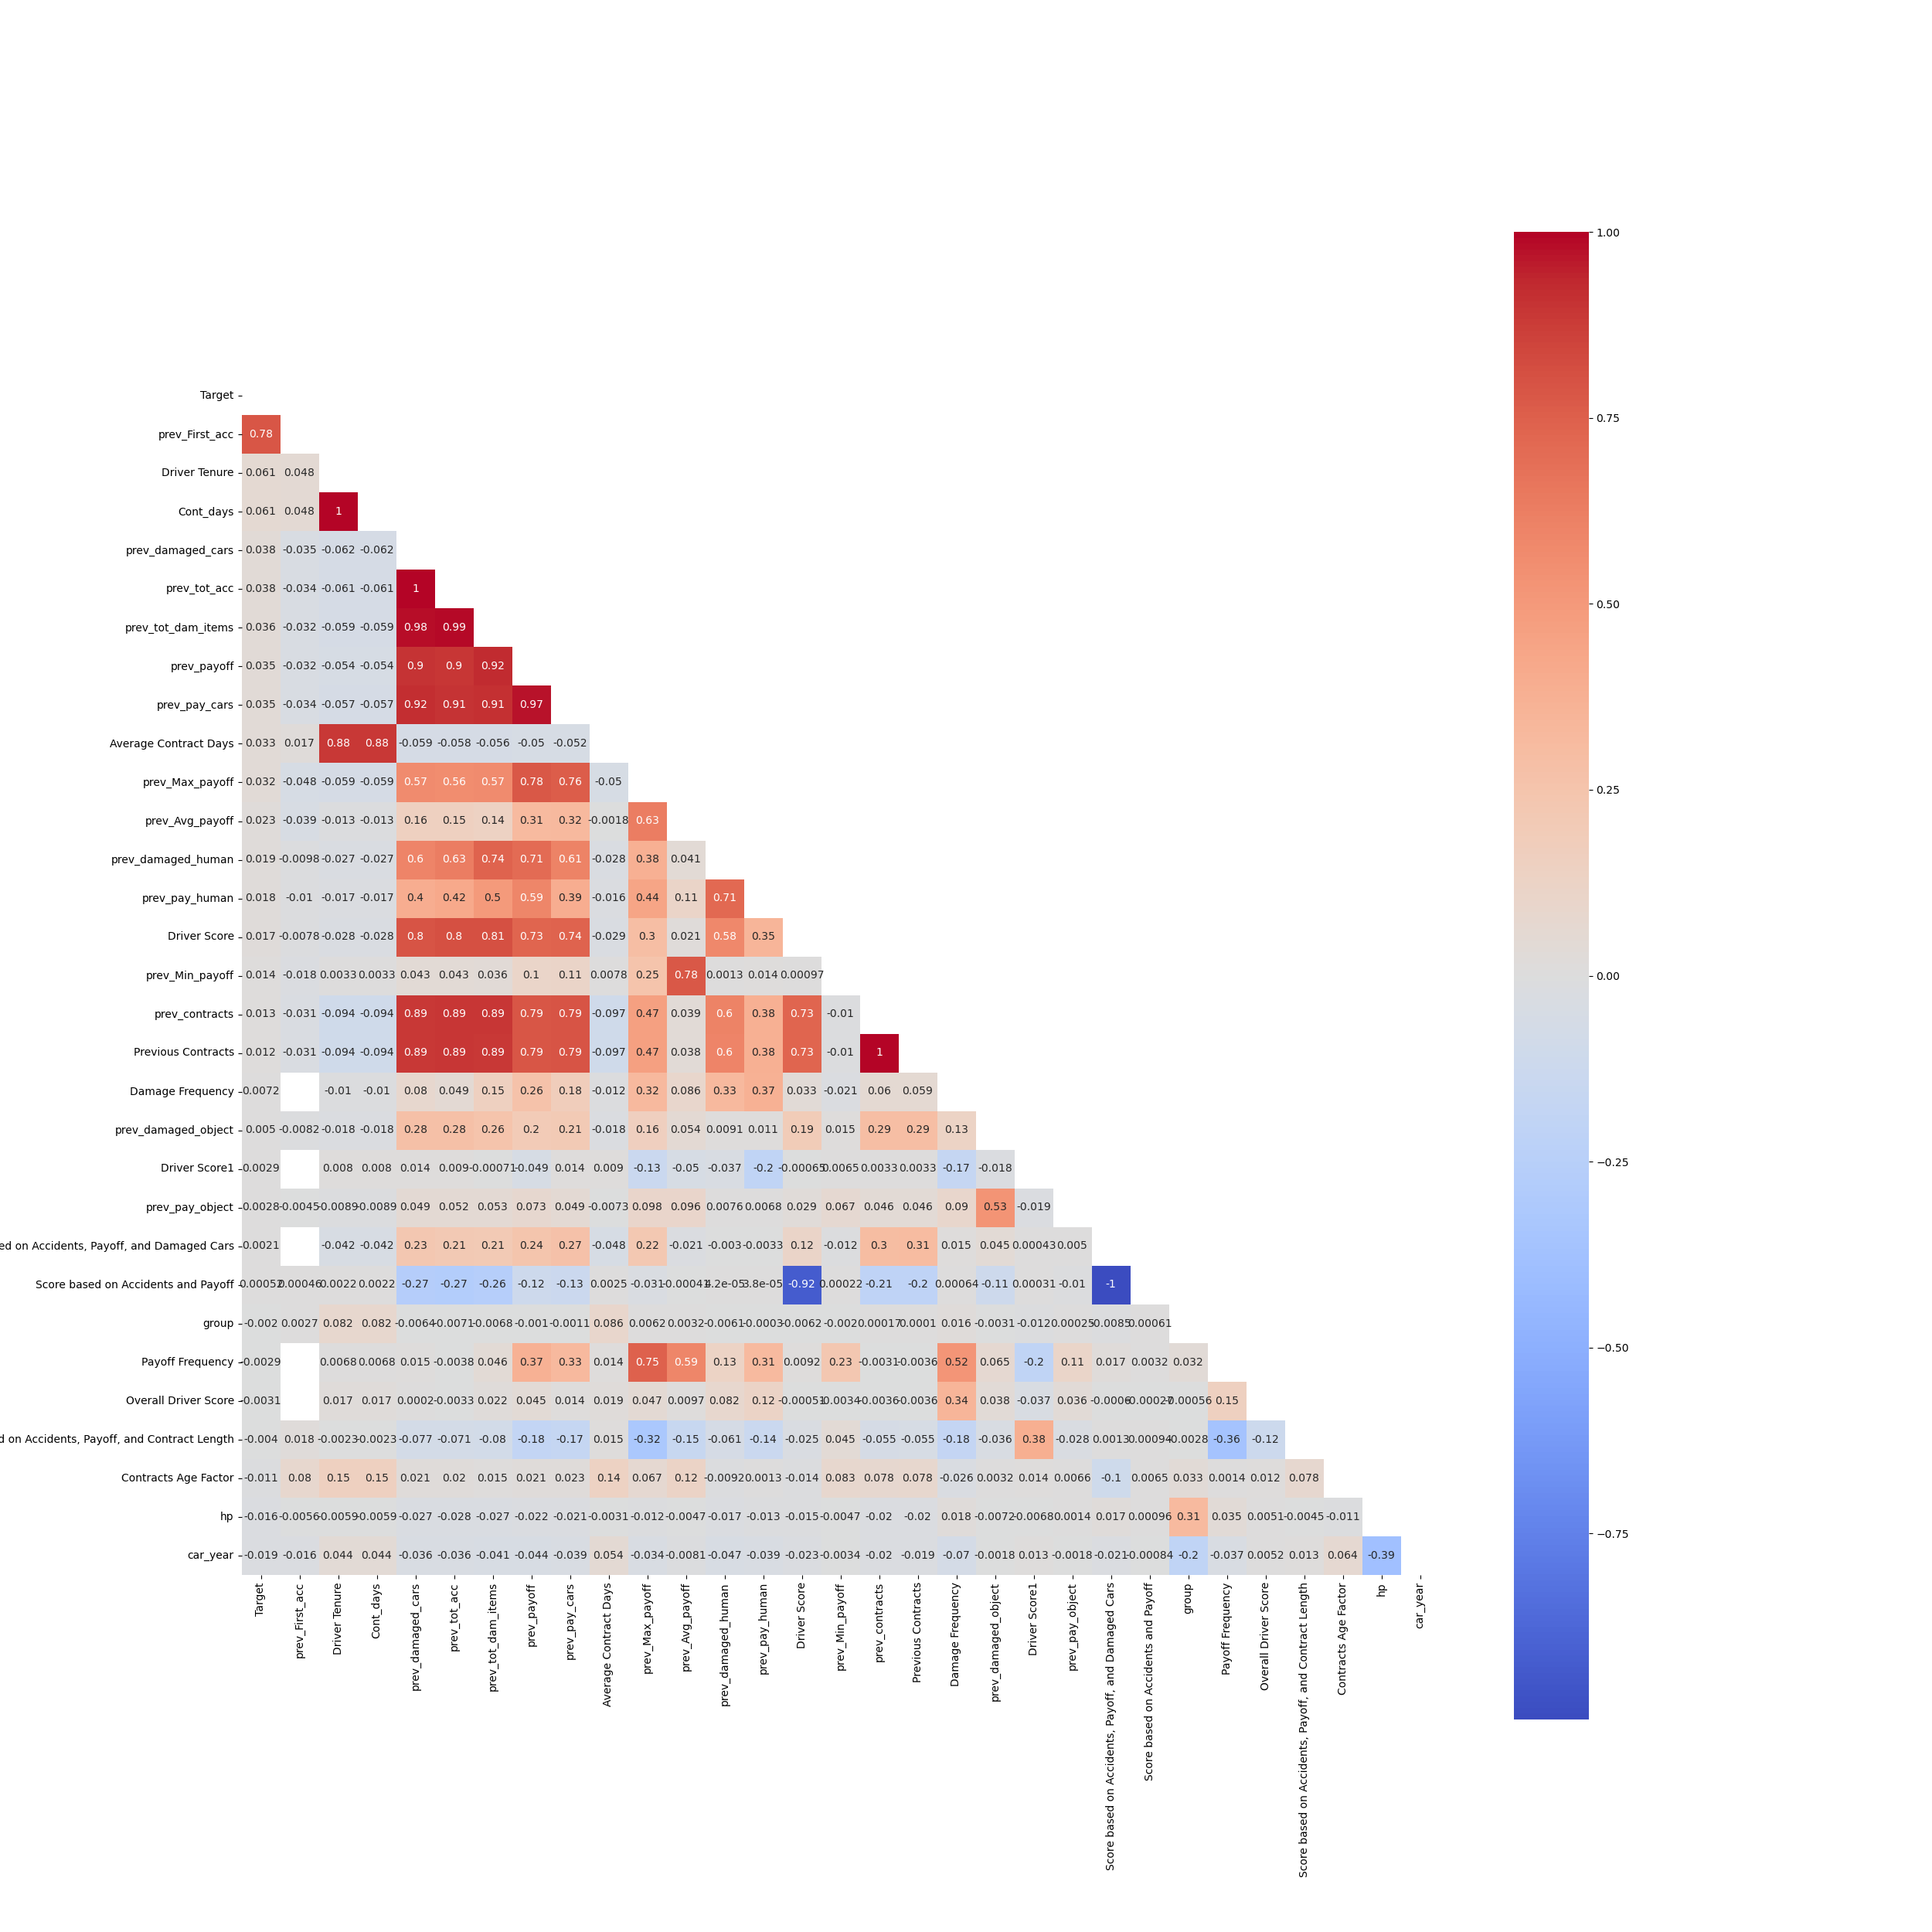
\includegraphics[width=0.5\textwidth]{cc.png}
\caption{\label{fig:cc}Data Correlation Matrix   }
\end{figure}


\section{Results }
\

\begin{figure}[htbp]
\centering
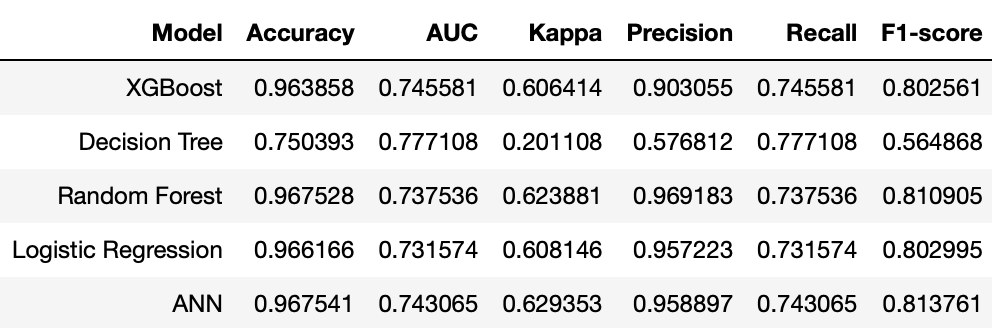
\includegraphics[width=0.45\textwidth]{res.png}
\caption{\label{fig:res}Ml model prediction results    }
\end{figure}



Based on the results of the machine learning models, we can conclude that the models are effective in predicting car accidents. The first model, XGBoost, achieved an accuracy of 96.39\text{\%}, indicating that it correctly predicted 96.39\text{\%} of the accidents. The precision and recall scores were 0.61 and 0.90, respectively, indicating that the model correctly classified 61\text{\%} of the accidents as positive and identified 90\text{\%} of the actual accidents. The F1-score of 0.80 indicates that the model achieved a good balance between precision and recall. Cohen's kappa score of 0.75 indicates substantial agreement between the predicted and actual labels. The second model, Decision Tree, achieved an accuracy of 75.04\text{\%}, precision, and recall scores of 0.20 and 0.58, respectively, and an F1 score of 0.56. Cohen's kappa score of 0.78 indicates substantial agreement between the predicted and actual labels. The third model, Random Forest, achieved an accuracy of 96.75\text{\%}, precision, and recall scores of 0.62 and 0.97, respectively, and an F1 score of 0.81. Cohen's kappa score of 0.74 indicates substantial agreement between the predicted and actual labels. The fourth model, Logistic Regression, achieved an accuracy of 96.62\text{\%}, precision, and recall scores of 0.61 and 0.96, respectively, and an F1 score of 0.80. Cohen's kappa score of 0.73 indicates substantial agreement between the predicted and actual labels. The fifth model, Artificial Neural Network, achieved an accuracy of 96.75\text{\%}, precision, and recall scores of 0.63 and 0.96, respectively, and an F1-score of 0.81. Cohen's kappa score of 0.74 indicates substantial agreement between the predicted and actual labels.


\begin{figure}[h]
\centering
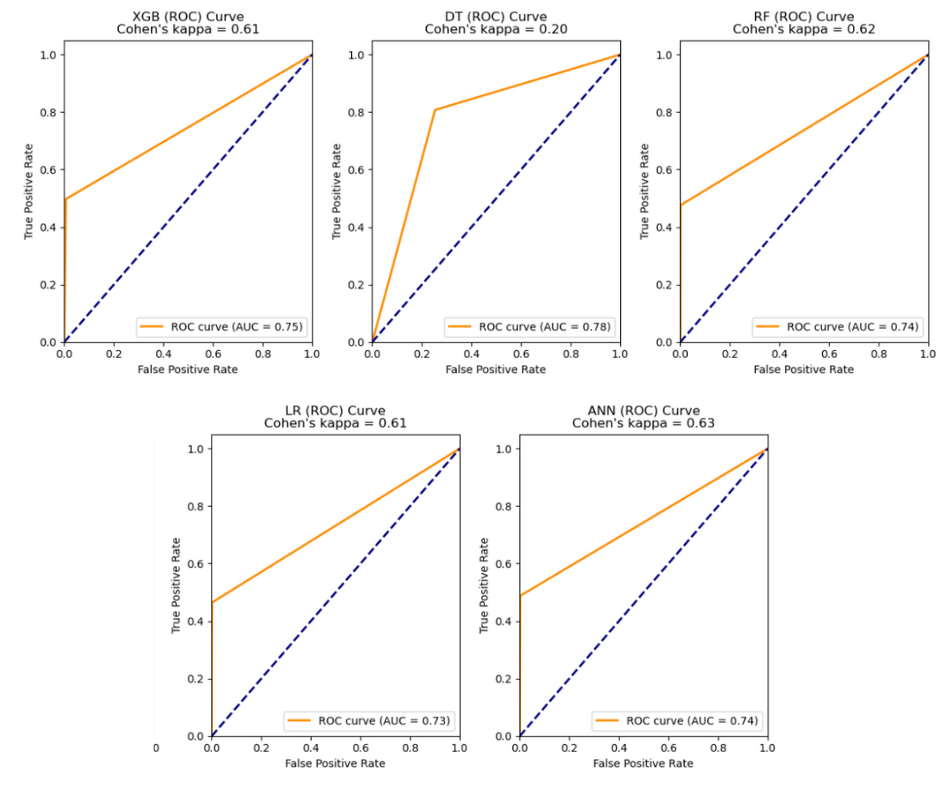
\includegraphics[width=0.35\textwidth]{aucc.png}
\caption{\label{fig:aucc}AUC curves for the models  }
\end{figure}

\section{Conclusion }

In this study, we apply ML algorithms to predict car accidents in the case of Armenia using a unique dataset from an Armenian insurance company. Based on the evaluation metrics, the best-performing models for car accident prediction are XGBoost and Artificial Neural Network, achieving the highest accuracy, precision, recall, F1- score, and Cohen’s kappa score. These models outperform the baseline Logistic regression model and the two other models: decision tree and random forest. The results can provide valuable insights for car insurance companies and policymakers to make better user decisions and policies. With the help of these models, car insurance companies can offer their customers more personalized policies based on their driving patterns and the likelihood of them getting into an accident. This would not only help to protect their customers better but also allow insurance companies to reduce costs and optimize their pricing policies. Further enhancement of the data can improve prediction accuracies. The extensions of this research can include the prediction of the number of accidents or the size of the damage (cost).


\bibliographystyle{plain}




\section{references }


\begin{itemize}

\item Baumgartner, J. (2021). Decision Trees for Machine Learning. Towards Data Science. \url{https://towardsdatascience.com/decision-trees-for-machine-learning-80d31e2cc263}
 \item Breiman, L. (2001). Random forests. Machine Learning, 45(1), 5-32. \url{https://doi.org/10.1023/A:1010933404324}
\item Breiman, L., Friedman, J. H., Olshen, R. A., \& Stone, C. J. (1984). Classification and Regression Trees. Chapman and Hall.
\item CDC. (2020). Motor Vehicle Crash Deaths. Retrieved from \url{https://www.cdc.gov/nchs/fastats/motor-vehicle-deaths.htm}
 \item Chen, T., \& Guestrin, C. (2016). XGBoost: A scalable tree boosting system. In Proceedings of the 22nd ACM SIGKDD International Conference on Knowledge Discovery and Data Mining (pp. 785-794). ACM. \url{https://doi.org/10.1145/2939672.2939785}
\item Columbus, L. (2018). Roundup Of Machine Learning Forecasts And Market Estimates, 2018. Forbes. \url{https://www.forbes.com/sites/louiscolumbus/2018/01/07/roundup-of-machine-learning-forecasts-and-market-estimates-2018/}
\item Fitch Ratings (2021). Fitch Ratings: Armenia insurance market report. Retrieved from \url{https://www.fitchratings.com/research/insurance/fitch-ratings-armenia-insurance-market-report-06-01-2021}
\item Géron, A. (2019). Hands-on machine learning with Scikit-Learn, Keras, and TensorFlow: Concepts, tools, and techniques to build intelligent systems. O'Reilly Media, Inc.
\item Gonçalves, M. A., Rocha, L. M., \& Lopes, L. S. (2012). The impact of training data quality on decision tree classifiers: An empirical study. Expert Systems with Applications, 39(1), 326-334.
\item Ministry of Finance of the Republic of Armenia (2021). Insurance market. Retrieved from \url{http://www.mfe.am/en/insurance-market}
\item National Safety Council. (2021). Motor Vehicle Fatality Estimates. Retrieved from \url{https://injuryfacts.nsc.org/motor-vehicle/overview/motor-vehicle-deaths-by-state-and-cause-2020/}
\item OECD (2018). Insurance market in Armenia: Overview and key challenges. Retrieved from \url{https://www.oecd.org/insurance/Insurance-Market-in-Armenia-Overview-and-Key-Challenges.pdf}
 \item Géron, A. (2019). Hands-on machine learning with Scikit-Learn, Keras, and TensorFlow: Concepts, tools, and techniques to build intelligent systems. O'Reilly Media, Inc.
\item Goodfellow, I., Bengio, Y., \& Courville, A. (2016). Deep learning. MIT Press.
\item Gonçalves, M. A., Rocha, L. M., \& Lopes, L. S. (2012). The impact of training data quality on decision tree classifiers: An empirical study. Expert Systems with Applications,
\item National Safety Council. (2021). Motor Vehicle Fatality Estimates. Retrieved from https://injuryfacts.nsc.org/motor-vehicle/overview/motor-vehicle-deaths-by-state-and-cause-2020/
\item OECD. (2018). Insurance market in Armenia: Overview and key challenges. Retrieved from https://www.oecd.org/insurance/Insurance-Market-in-Armenia-Overview-and-Key-Challenges.pdf
\item Wu, Y., Li, X., Li, Y., & Chen, X. (2017). Predicting car accidents using machine learning techniques. Journal of Physics: Conference Series, 847(1), 012044. https://doi.org/10.1088/1742-6596/847/1/012044
\item XGBoost. (n.d.). XGBoost: Scalable and flexible gradient boosting. Retrieved April 29, 2023, from https://xgboost.readthedocs.io/en/latest/
\item Zhang, C., & Liu, H. (2021). Decision Trees. In Z. Liu (Ed.), Encyclopedia of Database Systems (pp. 1-6). Springer. doi:10.1007/978-0-387-39940-9-465
\item "Predicting Traffic Accidents Using Convolutional Neural Networks with a Highway Camera" by D. I. Kim, K. W. Kim, and Y. B. Kim: https://www.mdpi.com/2076-3417/8/3/338/htm

\end{document}